\documentclass[tikz,border=3mm]{standalone}
\begin{document}

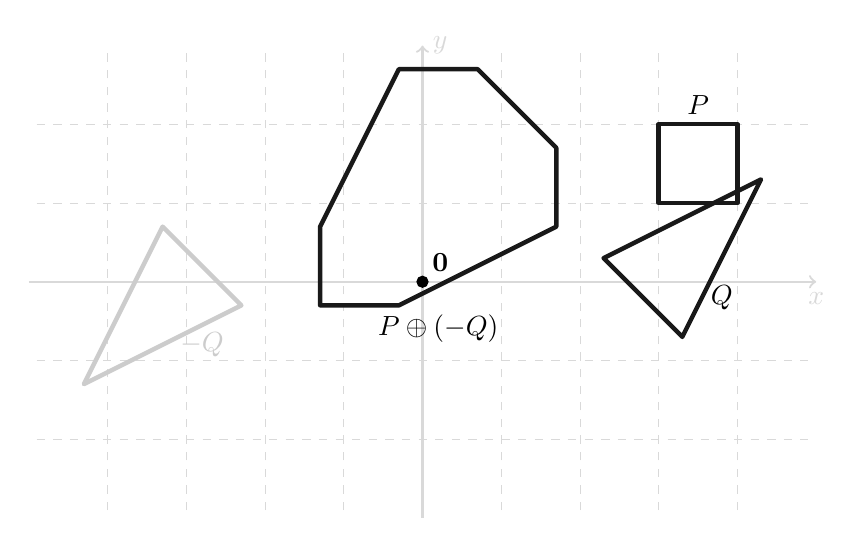
\begin{tikzpicture}
  % axes
  \draw[help lines, color=gray!30, dashed] (-4.9,-2.9) grid (4.9,2.9);
  \draw[->, thick, color=gray!30] (-5,0)--(5,0) node[below]{$x$};
  \draw[->, thick, color=gray!30] (0,-3)--(0,3) node[right]{$y$};

  % p
  \begin{scope}[shift={(3,1)}]
    \draw[ultra thick, color=black!90, line join=round] (0,0) -- (1,0) -- (1,1) -- (0,1) -- cycle;
    \draw (.5,1) node[above]{$P$};
  \end{scope}

  % q
  \begin{scope}[shift={(3.3,.3)}]
    \draw[ultra thick, color=black!90, line join=round] (-1,0) -- (0,-1) -- (1,1) -- cycle;
    \draw (.5,-.5) node{$Q$};
  \end{scope}

  % -q
  \begin{scope}[shift={(-3.3,-.3)}]
    \draw[ultra thick, color=black!20, line join=round] (1,0) -- (0,1) -- (-1,-1) -- cycle;
    \draw (.5,-.5) node[color=black!20]{$-Q$};
  \end{scope}

  % p + q
  \begin{scope}[shift={(-.3,0.7)}]
    \draw[ultra thick, color=black!90, line join=round] (-1,-1) -- (0,-1) -- (2,0) -- (2,1) -- (1,2) -- (0,2) -- (-1,0) -- cycle;
    \draw (0.5,-1) node[below]{$P \oplus (-Q)$};
  \end{scope}

  \filldraw[black] (0,0) circle (2pt) node[above right] {$\mathbf{0}$};
  
\end{tikzpicture}

\end{document}